% !TeX encoding = UTF-8
% !TeX program = pdflatex
% !TeX spellcheck = it_IT
\documentclass[binding=0.6cm]{sapthesis}
\usepackage{microtype}
\usepackage[italian]{babel}
\usepackage[utf8]{inputenc}
\usepackage{hyperref}
\usepackage{listings}
\usepackage{biblatex}
\addbibresource{bibliografia.bib}
%\lstset{basicstyle=\ttfamily, breaklines=true}
\usepackage{xcolor}  % Pacchetto per la gestione dei colori

% Impostazioni di base per lstlisting
\lstset{
    basicstyle=\ttfamily,  % Usa un font monospace per il codice
    backgroundcolor=\color{gray!10},  % Sfondo leggermente grigio
    frame=single,  % Aggiunge un bordo attorno al codice
    %caption={didascalia},  % Didascalia del blocco di codice
    captionpos=b,  % Posizione della didascalia (b = bottom, t = top)
    escapeinside={(*@}{@*)},  % Permette di aggiungere LaTeX all'interno del codice se necessario
}
\renewcommand{\lstlistingname}{fig.}


\hypersetup{pdftitle={La mia tesi},pdfauthor={Francesco Biccari}}
\title{Generazione e visualizzazione grafica di traffico di reti}
\author{Francesco Pannozzo}
\IDnumber{699427}
\course{Laurea Triennale in Informatica}
\courseorganizer{Facoltà di Ingegneria dell'Informazione, Informatica e Statistica}
\AcademicYear{2023/2024}
\advisor{Prof. Daniele De Sensi}
\authoremail{francesco.pannozzo@libero.it}
\copyyear{2024}
\thesistype{Relazione di tirocinio}
\begin{document}
\frontmatter
\maketitle
\dedication{Dedicato alla\\ mia famiglia}
\begin{abstract}
Questa relazione descrive il lavoro di tirocinio interno svolto presso l'università La Sapienza, 
concretizzato nella realizzazione 
di un progetto volto a realizzare un software per poter visualizzare in forma grafica l'andamento 
del traffico di una rete.
Il progetto ha come obiettivo di mostrare il traffico di rete al variare del tempo e ciò viene raggiunto
tramite grafiche e animazioni generate programmaticamente. L'idea dell'ambito di tirocinio nasce 
dalla volontà di sperimentare una realizzazione front-end tramite la libreria Manim, un motore di animazioni per video
matematici esplicativi..

\end{abstract}
\tableofcontents
\mainmatter
\chapter{Introduzione}
Nel mondo le reti informatiche sono oramai un concetto ben istanziato 
nella colletività, la loro presenza è soverchiante e si dirama nei più disparati settori.
Basti pensare già alle  reti PAN (Personal Area Network) le quali connettono dispositivi
personali entro pochi metri e che ognuno di noi usa abitualmente nella propria casa, 
alle reti LAN (Local Area Network), 
anch'esse presenti
nelle nostre case così come in uffici o edifici scolastici, le reti dei datacenter 
fino a giungere alla rete globale internet, la quale è creatrice a sua volta di paradigmi come
può essere l'internet of things. Le reti informatiche sono impiegate nei più vari 
settori come l'istruzione, in cui le reti
sono cruciali nelle scuole e nelle università per avere accesso a risorse educative o sfruttare l'e-learning, i servizi
pubblici governativi e sanitari, nel settore ludico e multimediale come il gioco online e l'attuale
streaming di contenuti multimediali: insomma, le reti informatiche sono di fatto una presenza piena e diffusissima
ed è estremamente difficile riuscire a immaginare il mondo come lo vediamo oggi senza questa tecnologia.
Con l'aumentare delle funzionalità legate alle reti, così come i dispositivi collegati a esse, capire cosa succede al
loro interno, come si muovono i dati, è quindi di cruciale importanza, tramite l'analisi dei dati che vi fruiscono è possibile fare diagnostica, per quanto
riguarda un discorso di monitoraggio, ma anche è possibile applicare le analisi in un ambito didattico e accademico.
Capire cosa sta succedendo in una rete in modo immediato e visivo è lo scopo di questo progetto, il quale punta a mostrare,
in modo grafico, l'andamento del traffico di una rete.
\section{Ambito del tirocinio}
Il progetto fa parte del percorso di tirocinio interno intrapreso presso l'Università La Sapienza di Roma. L'argomento su cui verte il progetto
è la realizzazione di un visualizzatore grafico dell'andamento del traffico di una rete, basato
su animazioni programmatiche. Il tool permette di visualizzare gli switch rappresentanti 
i vari endpoints e i link
che li collegano i quali vengono colorati tramite animazioni nel tempo in base al traffico di 
rete precedentemente analizzato. Nel tool è presente anche una parte generativa di traffico di rete,
una creazione di traffico fittizia di vitale importanza ai fini di testing.
\section{Motivazioni}
L'idea di sviluppare un visualizzatore grafico di traffico di rete è nata, 
in sede di proposta, dal Professore Daniele De Sensi, relatore del tirocinio, e dalla mia volontà di sviluppare un'applicazione avente il front-end
come focus dell'esperienza. Nel mio personale corso di studi presso il Dipartimento di Informatica non ho avuto modo
di studiare e approfondire un discorso legato al front-end, per cui la volontà di intraprendere questo percorso
nasce in primis da un forte interesse verso questo aspetto dell'informatica e in secondo luogo per un completamento di formazione professionale personale.
\section{Stato dell'arte}
L'esigenza di analisi di reti informatiche ha portato alla luce svariati tool che permettono
appunto di analizzare cosa avviene in una rete, di studiarne i dati statistici e di visualizzare
graficamente determinati scenari. L'universita americana Johns Hopkins\cite{JohnsHopkinsUniversity2024} ha stilato una lista
di software per la visualizzazione e analisi di reti\cite{JHUDatavisNetwork2024}:




\begin{itemize}
  \item \textbf{Gephi\cite{Gephi2024}:}
  Gephi è il software leader di visualizzazione ed esplorazione per tutti i tipi di grafici e reti ed è open source. Le sue caratteristiche includono
  l'analisi esplorativa dei dati mediante manipolazioni di reti in tempo reale, 
  analisi dei collegamenti per rivelare le strutture sottostanti delle associazioni tra oggetti, 
  analisi dei social network per la creazione di connettori di dati sociali per mappare le organizzazioni della comunità e le reti di piccoli mondi, 
  analisi della rete biologica per rappresentazione di modelli di dati biologici ed esportazione e 
  creazione poster erp promuovere e divulgare il lavoro scientifico con mappe stampabili di alta qualità.
  \item \textbf{Cytoscape\cite{Cytoscape2024}:} è una piattaforma software open source per visualizzare 
  reti complesse e integrarle con qualsiasi tipo di dati. Consiste in una piattaforma per
  visualizzare reti di interazioni molecolari e percorsi biologici, potendo integrare queste reti con annotazioni,
  profili di espressione genica e altri dati. Originariamente progettato per la ricerca biologica, 
  ora è una piattaforma generale per l'analisi e la visualizzazione di reti complesse.
  \item \textbf{GraphVis\cite{Graphviz2024}:} è un software di visualizzazione di grafici open source. Caratteristiche,
  I programmi di layout Graphviz accettano descrizioni di grafici in un semplice linguaggio di testo e creano diagrammi in formati utili, 
  come immagini e SVG per pagine web; PDF o Postscript per l'inclusione in altri documenti; 
  o visualizzare in un browser grafico interattivo. Graphviz ha molte funzionalità utili 
  per diagrammi concreti, come opzioni per colori, caratteri, layout di nodi tabulari, stili di linea, 
  collegamenti ipertestuali e forme personalizzate.
  \item \textbf{igraph\cite{igraph2024}:} è una collezione di librerie per creare, manipolare grafici e analizzare ponendo l'enfasi nell'efficienza,
  portabilità e facilità d'uso. Igraph è open source e gratuito e può essere programmato in R, Python, Mathematica e C/C++
  \item \textbf{UCINET6\cite{UCINET2024}:} è un pacchetto software per l'analisi dei dati dei social network. UCINET viene fornito con il tool di visualizzazione di rete NetDraw.
  Può leggere e scrivere una moltitudine di file di testo diversamente formattati, nonché file Excel. 
  I metodi di analisi dei social network includono misure di centralità, identificazione di sottogruppi, analisi di ruolo, teoria dei grafi elementari e analisi statistica basata sulla permutazione. 
  Inoltre, il pacchetto dispone di potenti routine di analisi delle matrici, come l'algebra delle matrici e la statistica multivariata.
  \item \textbf{SocNetV\cite{SocNetV2024}:}è un'applicazione software gratuita multipiattaforma per l'analisi e la visualizzazione dei social network.
  Tra le caratteristiche principali troviamo il poter disegnare i social network, caricare i campi da un file supportato
  (GraphML, GraphViz, Adjacency, EdgeList, GML, Pajek, UCINET, ecc.), personalizzare attori e collegamenti tramite sistema punta e clicca,
  analizzare le proprietà dei grafici e dei social network, produrre report HTML e incorporare layout di visualizzazione di rete
  \item \textbf{Pajek\cite{Pajek2024}:}  è un software per la visualizzazione e l'analisi delle reti. La sua forza risiede nel poter analizzare reti complesse potendo arrivare
  fino a un miliardo di vertici. L'analisi e la visualizzazione vengono eseguite utilizzando sei tipi di dati: 
  rete (grafico), partizione, vettore, cluster (sottoinsieme di vertici), permutazione (riordinamento dei vertici, proprietà ordinali); e gerarchia (struttura generale ad albero sui vertici).
\end{itemize}

\section{Contributi}
Da un punto di vista grafico e quindi di visualizzazione, la maggior parte degli strumenti sopra elencati, permette una certa forma di personalizzazione nella disposizione dei nodi, sia automaticamente attraverso algoritmi di layout sia manualmente, 
permettendo agli utenti di spostare i nodi per ottimizzare la visualizzazione o per enfatizzare certi aspetti della rete. Tuttavia, la possibilità di
avere animazioni dinamiche che mostrino l'andamento del traffico nel tempo, mostrando la variazione del colore in base alla quantità dello stesso, risulta
essere una caratteristica meno comune nei software di analisi di rete, nello specifico:
\begin{itemize}	
  \item Gephi: Non supporta nativamente animazioni dinamiche basate su traffico in tempo reale. Tuttavia, la sua flessibilità e la capacità di aggiungere plugin potrebbero permettere implementazioni personalizzate.
  \item Cytoscape: Anche se fortemente orientato all'analisi statica, plugin o estensioni potrebbero aggiungere capacità simili.
  \item GraphVis (Graphviz): Principalmente orientato verso la visualizzazione statica; non supporta direttamente animazioni dinamiche dei link basate sul traffico.
  \item igraph: Come libreria di analisi, non è orientato verso la visualizzazione in tempo reale o animazioni dei link basate su traffico nel suo utilizzo standard.
  \item UCINET (con NetDraw): Focalizzato sull'analisi statica di reti sociali; non supporta animazioni dinamiche in base al traffico.
  \item SocNetV: Orientato all'analisi statica e alla visualizzazione; non è progettato per visualizzare animazioni dinamiche basate sul traffico.
  \item Pajek: Simile agli altri, è più un tool per l'analisi statica e la visualizzazione di grandi reti, senza un supporto diretto per animazioni dei link basate su traffico.
\end{itemize}
In questo contesto, l'inserimento di una caratteristica che permetta di fare quanto premesso come base
del progetto di tirocinio, risulta particolarmente indicata nel contribuire a fornire una soluzione visiva come
strumento aggiuntivo di analisi di una rete, di debugging e anche come strumento didattico. La possibilità di
avere un riscontro visivo istantaneo di cosa avviene nel tempo in una rete, a livello di traffico, può dare immediato feedback nel
caso ci fosse un problema di congestione in un punto nevralgico, oppure mostrare parti di rete libere dove poter studiare un
reindirizzamento dello stesso, volto a ottimizzare le prestazioni. A livello didattico ciò si potrebbe mostrare per presentazioni così come per didattica tramite banalmente spiegazioni. 
Insomma i benefici derivanti da una rappresentazione del generale sono evidenti e ciò
può essere di grosso aiuto nell'analisi così anche solo come semplice rappresentazione del traffico di rete, nonchè uno strumento complementare a quanto già presente in circolazione.

\section{Base di partenza del progetto}
Il progetto è partito da zero, si basa sullo sviluppo totalmente nuovo dell'applicazione ed è stato tutto idealizzato e pianificato in sede di proposta.
Come approfondirò in seguito, nella sezione dedicata alla tecnologia impiegata, il progetto non è l'unica cosa a essere partita da zero, poichè il linguaggio
scelto per sviluppare l'applicazione è Python\cite{PythonWebsite}, linguaggio non incluso nel mio 
personale percorso di studi e che ho dovuto necessariamente studiare da zero per poter affrontare il percorso di tirocinio.

\chapter{Contesto di sviluppo: le tecnologie impiegate}
Il progetto, a livello di tecnologia impiegata, pone le fondamenta su tre aspetti, uno dei quali è
la scelta del linguaggio di programmazione che, come accennato precedentemente, è Python. Ci sono diversi validi motivi per cui 
puntare su questa tecnologia;
in primis è materia di insegnamento alla facoltà di Informatica de La Sapienza, ciò ha quindi una forte valenza accedemica, 
in secondo luogo risulta essere il linguaggio più
usato al mondo, ad affermarlo è l' Institute of Electrical and Electronics Engineers (IEEE)\cite{IEEEwebsite}\cite{IEEESpectrumArticle2023} 
un'associazione internazionale di scienziati professionisti con l'obiettivo della promozione delle scienze tecnologiche. Il linguaggio ha molte caratteristiche ottime, come
una sintassi semplice e leggibile che lo rende facile da imparare e semplice da usare per gli sviluppatori esperti accorciando di gran lunga i tempi di sviluppo,
una grande versatilità per poter essere usato in ambiti diversi come l'intelligenza artificiale, il web development, data analysys e molto altro, un ampio
supporto delle librerie, due delle quali usate proprio nel progetto (di cui ne parlerò a breve), una grande comunità in cui trovare facilmente risorse, tutorial e supporto,
una interoperabilità che permette un'ottima integrazione con altre tecnologie e altri linguaggi, orientato agli oggetti volto a facilitare la gestione del codice e migliora il riuso,
scalabile e di facile integrazizone. Il secondo aspetto risiede nella scelta della libreria Manim\cite{Manim}, che viene definita come "Animation engine for explanatory math videos". Lo scopo di Manim è quindi
quello di animare concetti tecnici legati alla matematica e si affida alla semplicità di Python per generare animazioni in modo programmatico. Manim può produrre anche immagini e gif, ma è nella produzione di video che splende, in questo modo
è possibile progettare animazioni e renderle visibili in movimento, coprendo figure algebriche, grafici cartesiani, grafi e molto altro\cite{Manim}. Manim viene impiegato principalmente per presentazioni che implichino aspetti matematici, la sfida del progetto è stata quella di 
cercare di sfruttare le potenzialità della libreria e renderle al servizio di uno strumento di analisi sul traffico di reti, una sfida vinta come potremo vedere in seguito.
Il terzo aspetto tecnologico riguarda l'aspetto di gestione dei dati. Un visualizzatore grafico di traffico di reti ha bisogno principalmente di due insiemi di informazioni importanti; uno riguarda tutte le informazioni
che riguardano il come è costruita la rate, parliamo quindi degli endpoint quali sono gli switch e conseguenti informazioni annesse, pensiamo ad esempio all'indirizzo di rete, un nome identificativo e così via, ma parliamo anche dei link che collegano
i vari endpoints, con la necessità di tenere traccia delle loro capacità trasmissive, la tipologia di rete, se ha una struttura a grafo completo, mesh, torus o disposizione libera e molte altre informazioni che discuteremo in seguito.
L'altro insieme di informazioni deriva dal traffico vero e proprio, rendendo quindi necessario un sistema di mantenimento dei dati legati ai pacchetti trasmessi. L'analisi di questi due insiemi di informazioni ha portato alla valutazione di tre sistemi per la strutturazione di dati; json\cite{RFC791}, yaml\cite{RFC9512} e csv\cite{RFC4180}.
Dopo attenta anlisi si è deciso di adottare il formato json per strutturare e memorizzare i dati legati al traffico, con la possibilità di scegliere anche il formato yaml, mentre per i dati relativi alla descrizione della rete il compito è stato affidato esclusivamente a yaml, csv è stato scartato.
Perchè csv è stato scartato? Sebbene csv rappresenti una valida alternativa tenendo conto di aspetti prestazionali, essendo un formato molto veloce da analizzare, da leggere e scrivere, tuttavia lo diventa meno quando c'è bisogno di strutturare maggiormente i dati con strutture più complesse dalla semplice forma tabellare, tipicamente usate nei database. 
L'idea di scartarla, sia per strutturare i dati della rete che per quelli del traffico, deriva principalmente dai seguenti motivi:

\begin{itemize}
    \item \textbf{Leggibilità:} uno dei primi intenti del progetto era di rendere l'applicazione il più leggibile possibile, questo perchè si è
    fortemente voluto attribuirne anche scopi di debugging e didattici, laddove avere una certa leggibilità è più che ragionevole.
    \item \textbf{Strutture complesse:} sicuramente il motivo più importante. Con csv non è possibile rappresentare strutture complesse, parliamo ad esempio di oggetti
    all'interno di altri oggetti. Sebbene per come sia ora strutturato il progetto una rappresentazione cvs è ancora possibile, ciò potrebbe non esserlo in futuro
    nell'ottica di espansione del progetto
\end{itemize}
Per esplicare meglio il concetto di struttura complessa non fattibile è possibile focalizzarsi sul seguente esempio. Segue la rappresentazione di diversi pacchetti così come sono utilizzati nel progetto:

\begin{lstlisting}[caption={pacchetti di rete rappresentati in json}]
    [
        {
            "A": 1,
            "B": 2,
            "t": "2024-03-22 12:30:00",
            "d": 1518
        },
        {
            "A": 2,
            "B": 1,
            "t": "2024-03-22 12:30:00",
            "d": 1518
        }
    ]
\end{lstlisting}
Dove A e B sono gli endpoints interessati, t è il timestamp di creazione pacchetto e d la dimesione del payload in bytes(). In csv questa struttura è rappresentabile come segue:
\begin{lstlisting}[caption={pacchetti di rete rappresentati in csv}]
    A,B,t,d
    2,1,2024-03-22 12:30:00,1518
    2,1,2024-03-22 12:30:00,1518
\end{lstlisting}
Tuttavia se si dovesse rendere questa struttura più complessa, avremmo problemi a realizzarla in csv, basterebbe l'aggiunta
di un campo che a sua volta necessita di informazione strutturata, come ad esempio inserire le informazione dell'header:
\begin{lstlisting}[caption={pacchetto di rete maggiormente strutturate in json}]
    [
        {
          "A": 1,
          "B": 2,
          "t": "2024-03-22 12:30:00",
          "d": 4000,
          "ip_header": {
            "version": 4,
            "ihl": 5,
            "type_of_service": 0,
            "total_length": 300,
            "identification": 98765,
            "flags": {
              "reserved_bit": false,
              "dont_fragment": true,
              "more_fragments": false
            },
            "fragment_offset": 0,
            "time_to_live": 64,
            "protocol": 6,
            "header_checksum": "2B5A",
            "source_address": "192.168.1.1",
            "destination_address": "192.168.1.2"
          }
        }
      ]
\end{lstlisting}
In questa struttura abbiamo ben due oggetti nidificati, ip header e flags. 
Questo tipo di struttura è difficilmente replicabile in csv che si presta maggiormente
per strutture piatte mentre json e yaml permettono molta più libertà di strutturazione.
La scelta del formato json per rappresentare i dati del traffico di rete è quindi legata alla possibilità di espandere la
rappresentazione con strutture più complesse in ottica di espansioni future del progetto, ma è indubbiamente legata alle prestazioni che questo formato riesce a dare.
Json è un formato ampiamente supportato e la sua semplicità permette di ottenere risultati ottimi per le operazioni di parsing, lettura e scrittura per strutture aventi grandi quantità di dati.
Per dare una stima approssimativa di grandezza, calcoliamo la quantità di pacchetti per secondo 
in un link con capacità di 1Gbps e relativa dimensione di un ipotetico file finale necessario
a memorizzare il tutto:
\begin{align*}
    \text{Capacità in bit} &= 10^9 \text{ bit} && \text{(1 gigabit)} \\
    \text{Capacità in bytes} &= \frac{10^9}{8} = 125,000,000 \text{ bytes} && \text{(1 byte = 8 bit)} \\
    \text{Dimensione massima del pacchetto} &= 1518 \text{ bytes} \\
    \text{Numero di pacchetti} &= \frac{125,000,000 \text{ bytes}}{1518 \text{ bytes per pacchetto}} \\
    &\approx 82345.19 && \text{(pacchetti)}\\
    \text{Bytes per pacchetto} &= 123 \text{ bytes} && \text{(Bytes per la scrittura su file)}\\
    \text{Numero righe di testo} &= 82345 \times 123 = 10128435 \text{ bytes}
    \end{align*}
Sebbene l'applicazione supporti sia json che yaml per quanto riguarda il memorizzare i dati legati al traffico, la scelta preferenziale ricade su json.
Questo perchè, nonostante json produca files di dimensioni maggiori rispetto a yaml, la schiacciante velocità di elaborazione di json rende la creazione di
un file di dimensioni maggiore ampiamente giustificabile, considerando soprattuto la natura del progetto in cui non vi è una
criticità d'uso nella dimensione dei files. Come vedremo in seguito, i test eseguiti sui tempi di lettura e scrittura rispettivamente della stessa struttura
ricreata sia in json che in yaml, sapranno ben
dimostrare quanto appena affermato.
Infinie giungiamo ai motivi per cui si è scelto invece esclusivamente yaml per rappresentare i dati relativi alle informazioni che descrivono la rete.

\chapter{Progettazione}

\chapter{Test}
Per ottenere i lati di un rettangolo che abbia proporzioni $16:9$ partendo da un 
quadrato di lato $n$, dobbiamo innanzitutto considerare che l'area del quadrato è data 
da $A = n^2$. Vogliamo che il rettangolo abbia la stessa area del quadrato ma rispetti
 le proporzioni $16:9$.

Denotiamo con $l$ la lunghezza e con $h$ l'altezza del rettangolo. La condizione di proporzione si può esprimere come
\[
\frac{l}{h} = \frac{16}{9}.
\]
Dato che l'area del rettangolo deve essere uguale a quella del quadrato, abbiamo che
\[
l \cdot h = n^2.
\]
Utilizzando la proporzione, possiamo esprimere $l$ in termini di $h$ come
\[
l = \frac{16}{9}h.
\]
Sostituendo questa espressione nell'equazione dell'area, otteniamo
\[
\frac{16}{9}h \cdot h = n^2,
\]
che si semplifica in
\[
\frac{16}{9}h^2 = n^2.
\]
Da qui, isoliamo $h$ ottenendo
\[
h^2 = \frac{9}{16}n^2 \quad \Longrightarrow \quad h = n \cdot \frac{3}{4}.
\]
Risostituendo il valore di $h$ nell'espressione di $l$, abbiamo
\[
l = \frac{16}{9} \cdot n \cdot \frac{3}{4} = n \cdot \frac{4}{3}.
\]
Quindi, per un quadrato di lato $n$, per ottenere i lati di un rettangolo che mantenga la stessa area ($n^2$) con proporzioni $16:9$, l'altezza $h$ del rettangolo sarà $n \cdot \frac{3}{4}$ e la lunghezza $l$ sarà $n \cdot \frac{4}{3}$.



Quindi il tutto funziona poichè è sempre vero quanto segue:
\begin{equation}
(l+1)(m+1)>ml
\end{equation}

\section{Sotto capitolo test}

Ecco un esempio di codice YAML:

\begin{lstlisting}
- coordinates:
    - [1, 2]
    - [3, 0]
\end{lstlisting}

E ora un esempio di codice Python:

\begin{lstlisting}[language=Python]
links = {}
# Extracting links data
for content in networkData[CONST.NETWORK["LINKS"]]:
    links[frozenset({content["endpoints"][CONST.EP_A], content["endpoints"][CONST.EP_B]})] = {
        #"linkID": link,
        "capacity": content["capacity"], 
        "trafficDT":0, 
        "trafficUDT":0, 
        "updateDeltaTraffic": [], 
        "traffic": []
        }
\end{lstlisting}
La complessità temporale dell'algoritmo è $O(m+n)$.
\begin{equation}
    O(m+n)
\end{equation}

.. .. ..
\begin{figure}[h]
    \centering
    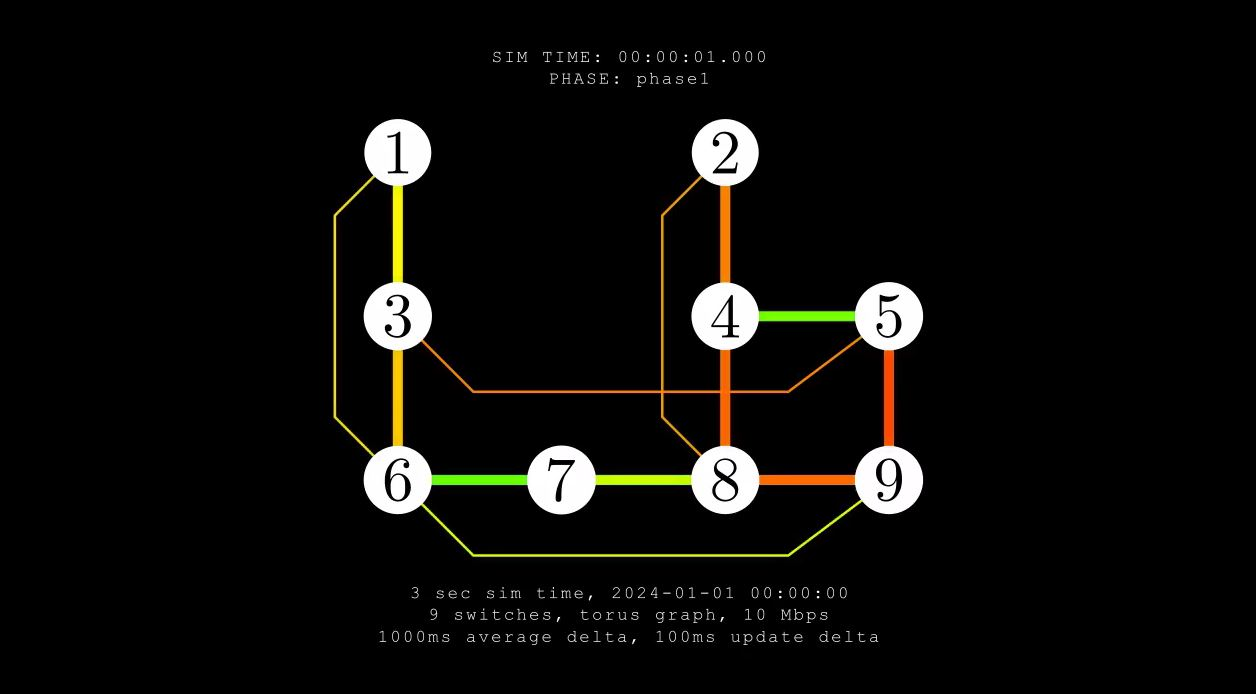
\includegraphics[width=0.8\textwidth]{immagini/only_links.JPG}
    \caption{a nice plot}
    \label{fig:only_links}
\end{figure}

As you can see in the figure \ref{fig:only_links}, the 
function grows near 0. Also, in the page \pageref{fig:only_links} 
is the same example.


\printbibliography

\backmatter
\cleardoublepage
\phantomsection % Give this command only if hyperref is loaded
\addcontentsline{toc}{chapter}{\bibname}
% Here put the code for the bibliography. You can use BibTeX or
% the BibLaTeX package or the simple environment thebibliography.
\end{document}